\documentclass[a4paper,11pt,oneside]{book}

\usepackage{float}
\usepackage{graphicx}
\usepackage{longtable}
\usepackage{multirow}
\usepackage{CJK}
\usepackage{listings}
\usepackage{xcolor}
\usepackage{fancyhdr}
\usepackage{indentfirst}
\usepackage{amsmath}
\usepackage{enumerate}
\usepackage{wasysym}
\usepackage[font=small,format=plain,labelfont=bf,up,textfont=it,up]{caption}
\usepackage[body={14cm,22cm},bindingoffset=2cm]{geometry}
\usepackage[
	dvipdfm,
	CJKbookmarks=true,
	bookmarksnumbered=true,
	bookmarksopen=false,
	colorlinks,
	linkcolor=black
	]{hyperref}

\pagestyle{fancy}
\setlength{\skip\footins}{1cm}
\setlength{\headheight}{-1cm}

\renewcommand{\footnotesize}{}
\renewcommand{\footrulewidth}{0pt}

\setlength{\unitlength}{2em} % for the picture environment

% 4 levels of headings
\newcommand{\headA}[1]{{\huge \vspace{1ex} \bf \hfill #1 \vspace{1ex}\hfill}}
\newcommand{\headB}[1]{{\Large \vspace{1ex} \bf #1 \vspace{1ex} }}
\newcommand{\headC}[1]{{\large \vspace{1ex} \bf #1 \vspace{1ex} }}
\newcommand{\headD}[1]{{\bf \vspace{1ex} #1 \vspace{1ex} }}

\newcommand{\pushin}{\hspace*{1em}}

\lstdefinelanguage{mwshell}{
	morekeywords={if,then,elif,else,fi,for,in,while,do,done},
	morecomment=[l]{\#\ },
}

\lstset{
	numbers=left,
	%framexleftmargin=10mm,
	%frame=none,
	%frame=shadowbox,
	%rulesepcolor=\color{blue},
	backgroundcolor=\color[RGB]{200,200,200},
	tabsize=4,
	breaklines=true,
	keywordstyle=\bf\color{blue},
	%identifierstyle=\bf,
	%numberstyle=\color[RGB]{0,192,192},
	commentstyle=\it\color[RGB]{0,96,96},
	%stringstyle=\rmfamily\slshape\color[RGB]{128,0,0},
	showstringspaces=false,
	lineskip=0.5pt,
	basicstyle=\ttfamily\small
}

\setlength{\parindent}{2em}


\title{g-bios开发者手册(第1卷,使用入门)}
\author{MaxWit魔鬼训练营}

%\renewcommand{\baselinestretch}{1.3}
\linespread{1.3}

\pagestyle{fancy}

%\lhead[g-bios开发者手册(第1卷)]{\leftmark}
\chead{}
\rhead{\href{http://www.maxwit.com}{g-bios开发者手册(第1卷)}}

\fancyfoot{}
\cfoot{\thepage}

\newcounter{count}
\newcommand{\RefCount}{\arabic{count}\refstepcounter{count}}

\begin{document}
\maketitle

\frontmatter
\tableofcontents

\mainmatter

\chapter{初识g-bios}
\section{g-bios简介}
%\section{g-bios: An Open Source Bootloader Project}
%MaxWit开放实验室(MaxWit Open Lab)是由多家公司资助成立的,致力于研发开源项目和探讨软件开发技术的公益性组织。2008年1月正式成立于上海浦东张江高科,目前开放实验室成员主要来源于Google、Intel、 TI、AMD、华为、Cisco、飞利浦等公司资深研发人员以及清华、浙大、上交大、中科院等科研院校的师生。

g-bios(以下简称g-bios)是由Intel、IBM、Qualcomm、AMD等公司的几名软件工程师与开源社区共同研发的一个Bootloader\footnote{或者说是一个嵌入式系统的BIOS,相当于PC机的BIOS+Bootloader。}。g-bios不但借鉴了几乎所有主流BSP/BIOS/Bootloader的优点,而且加入不少独创的特性,包括:
\begin{enumerate}\setlength{\itemsep}{-\itemsep}
\item 自动检测有待烧录的image文件类型,并智能自动烧录。
\item 支持多种文件系统,包括YAFFS2、JFFS2、CRAMFS、UBI、NFS等。
%\item 支持两种用户界面:GUI(类似传统PC BIOS)和命令行模式(面向嵌入式系统)。
\item 命令行自动补全(Tab)键及历史记录(上、下键)支持。
\item Flash(MTD)分区支持,帮助Linux、Android内核识别分区。
\item 自动设置Linux内核启动参数(Linux kernel command line),极大地降低了参数设置的复杂度并减少了启动出错的概率。当然,同时也支持手动设置,以满足特殊要求。
\item 常用命令具有记忆功能。如boot命令,它能记住用户输入的参数,以后只需简单输入boot即可。
\item 引入全新的架构及NB技术(即Never Burn-down,又称``烧不死''技术)。
%核心设计思想是:把g-bios分为上半部分和下半部分,上半部分以最小的代码量完成CPU和Memory的初始化,并实现引导下半部分的功能;下半部分为g-bios主体。上半部分设计简单,调试周期短,完成后就固化在特定的引导区中不再更改;
开发人员可在没有仿真器的情况下大胆开发
Bootloader
%下半部分代码(即g-bios%主体)
。事实上,只需一根串口数据线应能轻松完成整个g-bios的开发。启动代码的地址无关性带来的麻烦?没有了!因为bug或不小心改错了代码,甚至是数据线连接问题而导致启动黑屏?也不可能出现了!
%在调试完成并正试发布的产品时,若有必要,也可将上下两部分可合成一个整体——只需一个命令重新编译即可。
\item 支持完整的中断机制。开发者可简单地通过一个编译选项选择IRQ或Polling两种模式的中的任意一种。
\item 优秀的网络子系统,并提供符合POSIX规范的Socket API,方便二次开发。
%\item 优秀的软件架构及子系统设计,包括:中断、网络、Flash、USB子系统,等等。
%\item 集成类似PC机版本的Video BIOS。
%\item 支持基于龙芯的PC机及嵌入式系统。
\item 支持
%嵌入式系统几乎所有
多种常用外设,包包括:WDT、UART、NAND、NOR、SD/MMC、USB、LCD、Touchscreen,...
\item 集成硬件调试/测试程序,大大提高了bring-up的工作效率。
\item 完美支持Google Android操作系统,简化Android的系统移植过程。
\item 支持图形化配置,不但让新手很容易上手,而且使g-bios的移植和开发过程变得更简单。
\end{enumerate}

更多详情,请登录项目主页http://maxwit.googlecode.com或ChinaUnix论坛上的g-bios版块(http://bbs.chinaunix.net/forum-238-1.html)。

\section{获取g-bios源码}
请确认git(一个版本管理软件)已经安装,然后执行如下命令:
\begin{lstlisting}[language=bash,numbers=none]
$ git clone git://github.com/maxwit/g-bios.git
\end{lstlisting}
此时会在当前目录(方便描述起见,假定为HOME目录)下将会创建一个名为 ``g-bios''的目录,该目录中为g-bios源码。
%\section{如何参与g-bios开发}
%g-bios开源社区采用maillist和bbs相结合的方式,任何人都可以通过这两种方式把自己的代码递交给g-bios项目维护者。若对文档有任何疑问或改进也可联系我们。
%  \begin{table}[htbp]
%  \centering
%  \setlength{\parindent}{0pt}
%  \begin{tabular}{|c|c|}
%  \hline
%  g-bios论坛 &\small http://linux.chinaunix.net/bbs/forum-70-1.htm \\
%  \hline
%  g-bios邮件列表 &\small maxwit@googlegroups.com \\
%  \hline
%  g-bios项目维护者 &\smallConke Hu $<$conke.hu@gmail.com$>$ \\
%					 &\smallTiger Yu $<$tigerflying.yu@gmail.com$>$ \\
%					 &\smallFleya Hou $<$fleya.hou@gmail.com$>$ \\
%  \hline
%  文档编辑 &\small  \\
%  \hline
% \end{tabular}
% \end{table}

\section{g-bios体系结构}
% figure


\chapter{g-bios的编译及烧录}
\section{g-bios配置}
与编译Linux kernel类似,进入在g-bios源码目录,执行make PLAT\_defconfig(PLAT指的是具体硬件平台名称,例如s3c6410\_defconfig或者beagle\_defconfig, g-bios所支持的各硬件平台的默认配置文件位于g-bios源码build/configs目录下),用默认的选项编译g-bios,然后执行make进行编译,如需要将编译产生的image文件拷贝到tftpboot目录下,还需要执行make install命令。如果需要修改默认的编译选项,可以直接执行make menuconfig,在随后出现的GUI中进行配置。目前的2.5版本暂不支持GUI配置方式。

\subsection{基于命令行的配置方式}
切换到g-bios源码目录下,然后执行如下命令:
\begin{lstlisting}[language=bash, numbers=none]
$ make ${BOARDNAME}_defconfig
\end{lstlisting}
其中BOARDNAME为某个具体的硬件平台名称,如beagle、mw61、mini2440等。

\subsection{基于图形界面的配置方式}
切换到g-bios源码目录下,然后执行如下命令:
\begin{lstlisting}[language=bash, numbers=none]
$ make menuconfig
\end{lstlisting}

\subsection{配置选项详解}
接下来分析一个各个配置选项的功能作用。

Platform:	g-bios运行的platform,可以是at91sam9263、at91sam9261、s3c2410、s3c2440或s3c6410等,这是目前g-bios支持的几个Platform。Toolchain:编译g-bios源码所选用的编译工具,默认使用的是lablin源码包编译生成的toolchain,也可以手工修改为系统上已有的toolchain(注:Toolchain要支持EABI)。Image Patch编译g-bios后生成的image路径,默认为/var/lib/tftpboot目录。Server IP服务器IP,local IP开发板IP,将二者设为同一网段。此二项,也可不配。MAC Addr此项不用理会,Nfs Path:g-bios引导内核时,如用nfs加载rootfs时,指定rootfs路径,默认路径$\sim$/maxwit/rootfs。Flash ECC mode选择ECC校验模式(硬件ECC,软件ECC,也可不使用ECC)。IRQ/Polling Mode g-bios使用中断模式还是非中断模式(Polling)。

g-bios配置程序所完成的功能:
\begin{table}[htbp]
\centering
\setlength{\parindent}{0pt}
\begin{tabular}{|c|l|l|}
\hline
类别 & \multicolumn{1}{|c|}{选项} & \multicolumn{1}{|c|}{功能说明} \\ \hline
\multirow{3}{*}{general} & Platform & g-bios运行的目标Platform \\ \cline{2-3}
		& TooLchain & 编译g-bios的编译工具 \\ \cline{2-3}
		& Image Path & 编译生成image的目录 \\ \hline
\multirow{4}{*}{Network} & Server IP & 服务器IP \\ \cline{2-3}
		& Local IP & 目标机IP \\ \cline{2-3}
		& MAC addr & MAC地址\\ \cline{2-3}
		& NFS root path &  lablin的rootfs路径\\ \hline
\multirow{3}{*}{Flash ECC Mode}   & Hardward & 支持硬件ECC\\ \cline{2-3}
		& Software & 软件ECC\\ \cline{2-3}
		& None & 无ECC较验\\ \cline{2-3}
\multirow{2}{*}{IRQ/Polling Mode} & IRQ Enabled & 支持中断 \\ \cline{2-3}
		& Polling Mode & 查询模式(非中断)\\ \hline
\end{tabular}
\end{table}

%\begin{itemize}
%\item Gerneral
%\item Tophalf
%\item Uart
%\item Memory
%\item Flash
%\item NetWork
%\item Interrupt
%\item Logo
%\item Boot
%\end{itemize}

\section{编译}
%\subsection{``make'' and ``make install''}
上面通过configure配置的g-bios编译特性,生成了Makefile。本节将编译g-bios。
\begin{lstlisting}[language=bash,numbers=none]
$ make
$ make install
\end{lstlisting}
编译后会在/var/lib/tftpboot(configure中配置的Image Path)目录下生成witrom.bin和g-bios.bin二个文件。


%\chapter{g-bios的烧录}
\section{烧录}
\subsection{Burning Top-Half}
g-bios上半部分的烧录方法与其他的bootloader一样,都依赖于具体的板子,请大家参考板子的手册烧录TH。
g-bios上半部主要是Load下半部,为下半部服务。Load BH的方式有如下几种:
\begin{enumerate} \setlength{\itemsep}{-\itemsep}
\item 从串口下载下半部并运行
\item 从Flash上Load下半部并运行
\item 自动检测Flash上的下半部是否存在,若存在则默认从Flash上Load下半部并运行,否则等待从串口Load。
\end{enumerate}

\subsection{烧录g-bios BH(下半部分)}
上电或重起后,连接任意键可即可进入g-bios TH的引导菜单。若不按键刚TH默认从Nand Flash中Load BH并执行将执制权交给BH。通过TH Load BH的菜单如下所示:
\begin{figure}[H]
\centering
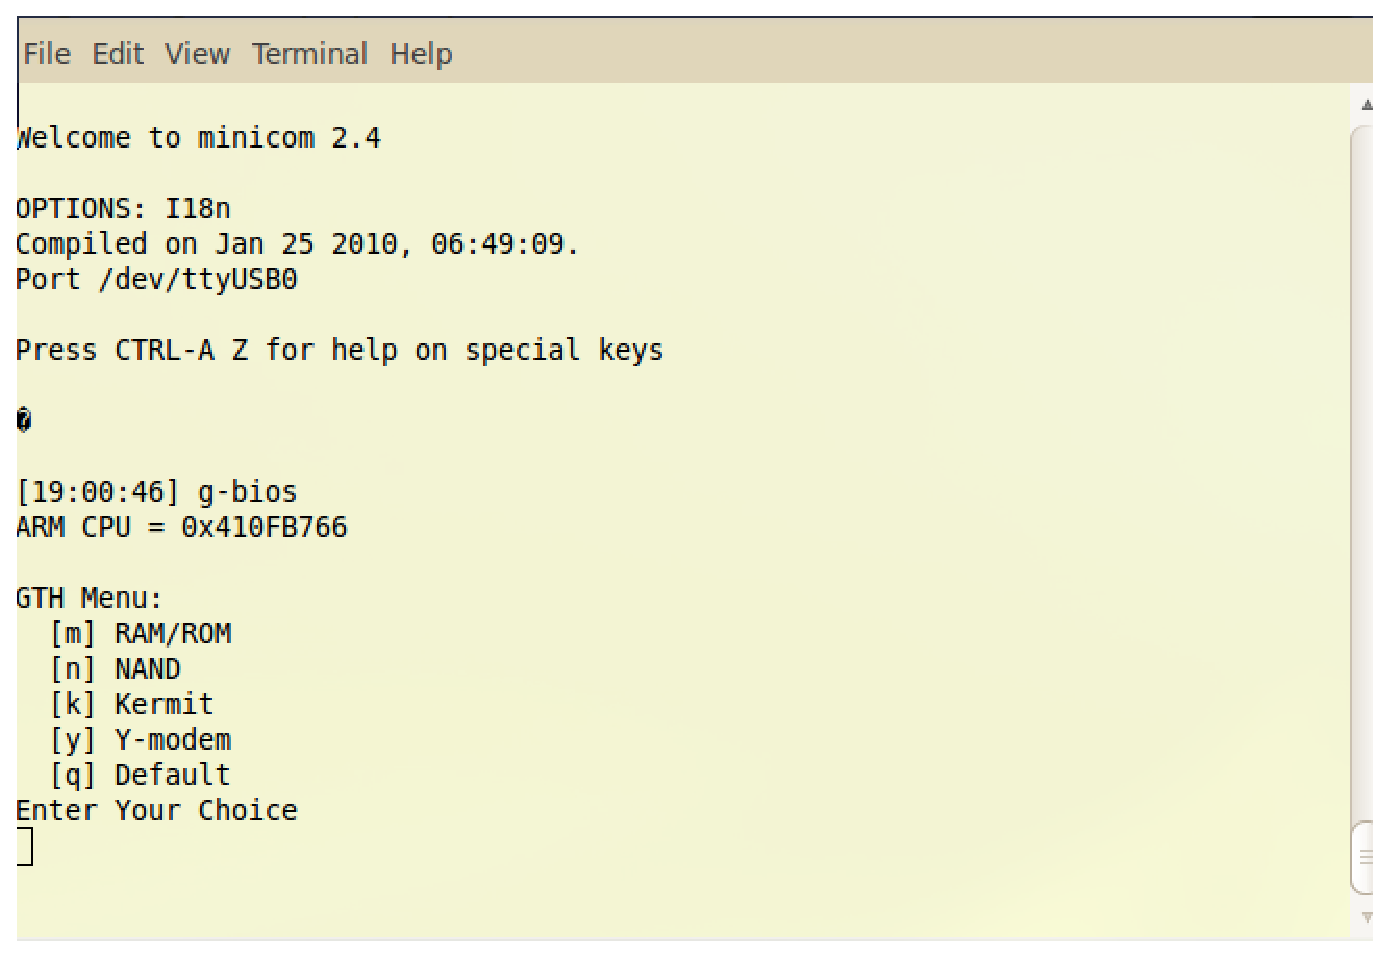
\includegraphics[width=0.8\textwidth]{image/min_01.eps}
\end{figure}
选择不同的选择即可以不同的方式Load BH。以Kermit和Minicom为例从串口引导g-bios bh。
\begin{enumerate} \setlength{\itemsep}{-\itemsep}
\item Ymodem:(注意:minicom在以下过程中要求使用速度很快。)
	\begin{enumerate} \setlength{\itemsep}{-\itemsep}
	\item 连接电源,串口线(开发板上的COM1),网线。
	\item 打开minicom软件。
	\begin{lstlisting}[language=c,numbers=none]
	$ minicom
	\end{lstlisting}
	\item 按下空格键(一直接)。打开电源开关。
	\begin{figure}[H]
	\centering
	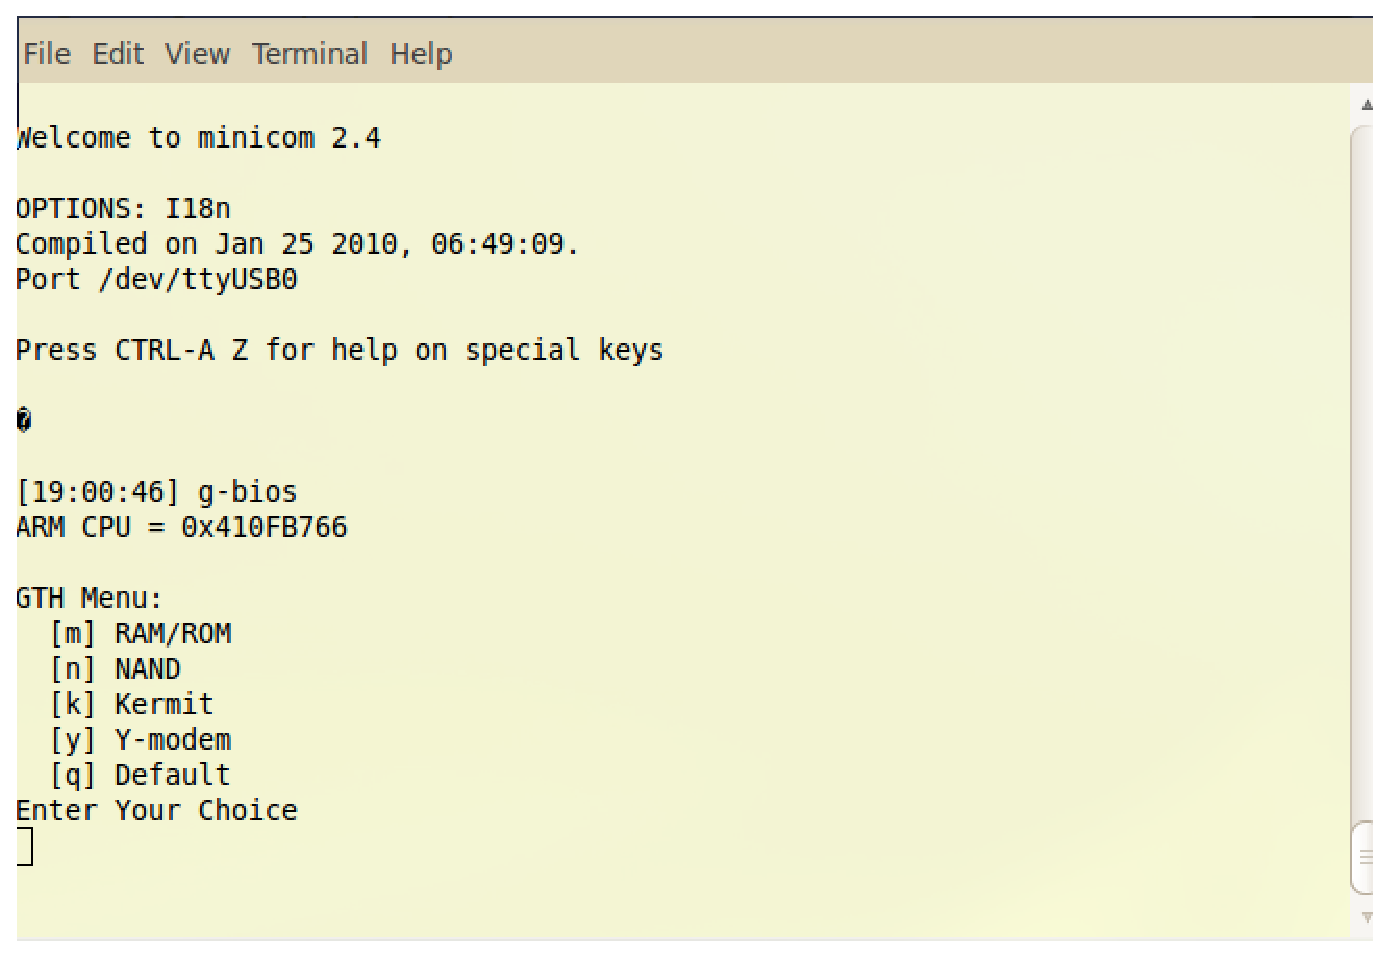
\includegraphics[width=0.8\textwidth]{image/min_01.eps}
	\end{figure}
	\item 按下'Y'键
		\begin{figure}[H]
		\centering
		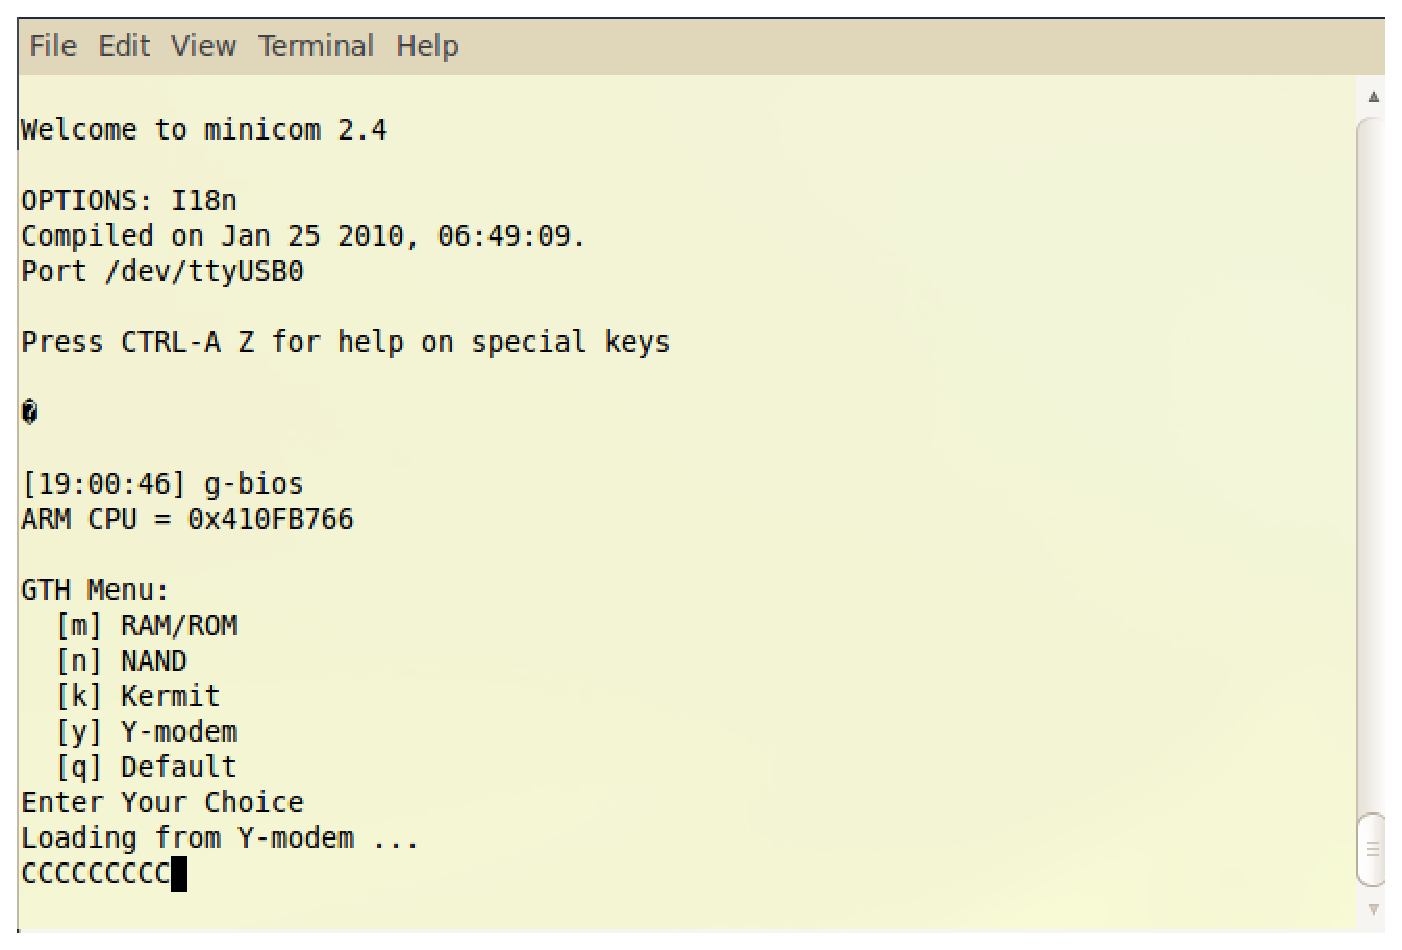
\includegraphics[width=0.8\textwidth]{image/min_02.eps}
		\end{figure}
	\item 同时按下``Ctrl'' + 'a', 再按's'.
		\begin{figure}[H]
		\centering
		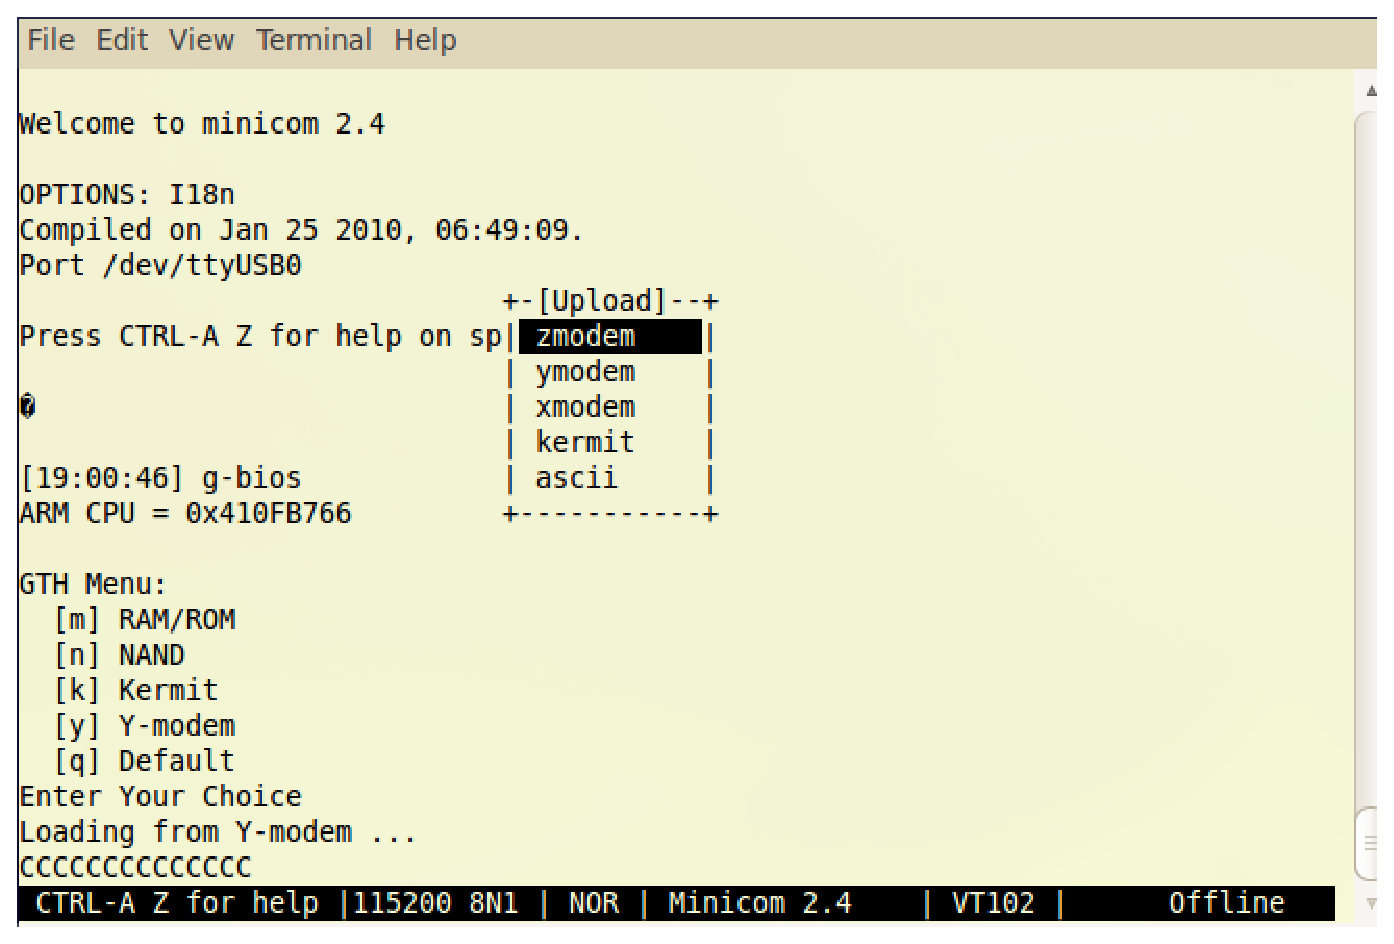
\includegraphics[width=0.8\textwidth]{image/min_03.eps}
		\end{figure}
	\item 用方向键选择``ymodem'',回车。
		\begin{figure}[H]
		\centering
		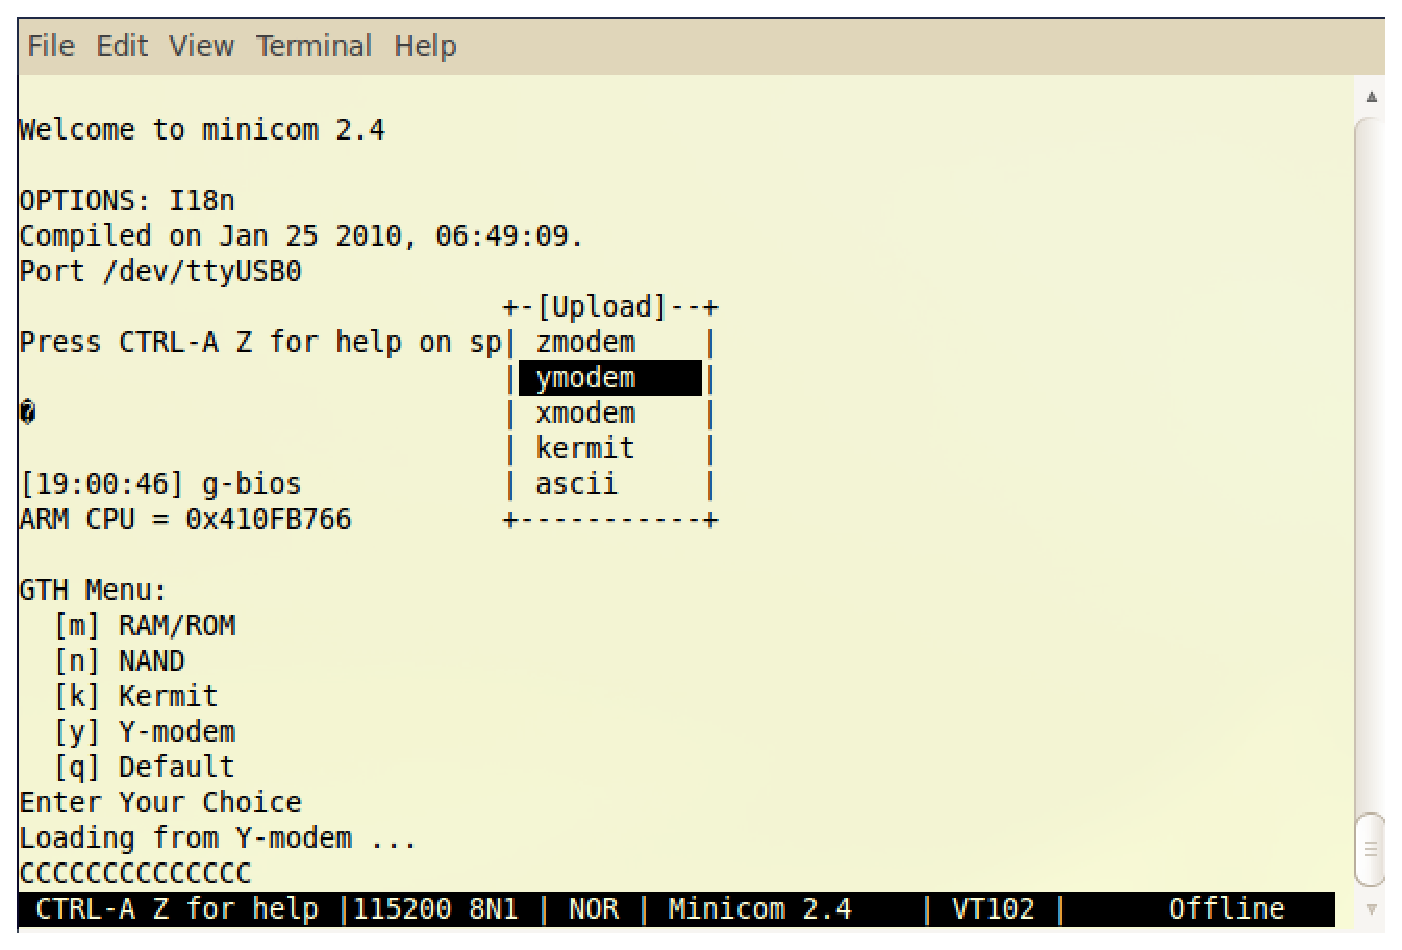
\includegraphics[width=0.8\textwidth]{image/min_04.eps}
		\end{figure}
	\item 选择``Okay'',回车。
		\begin{figure}[H]
		\centering
		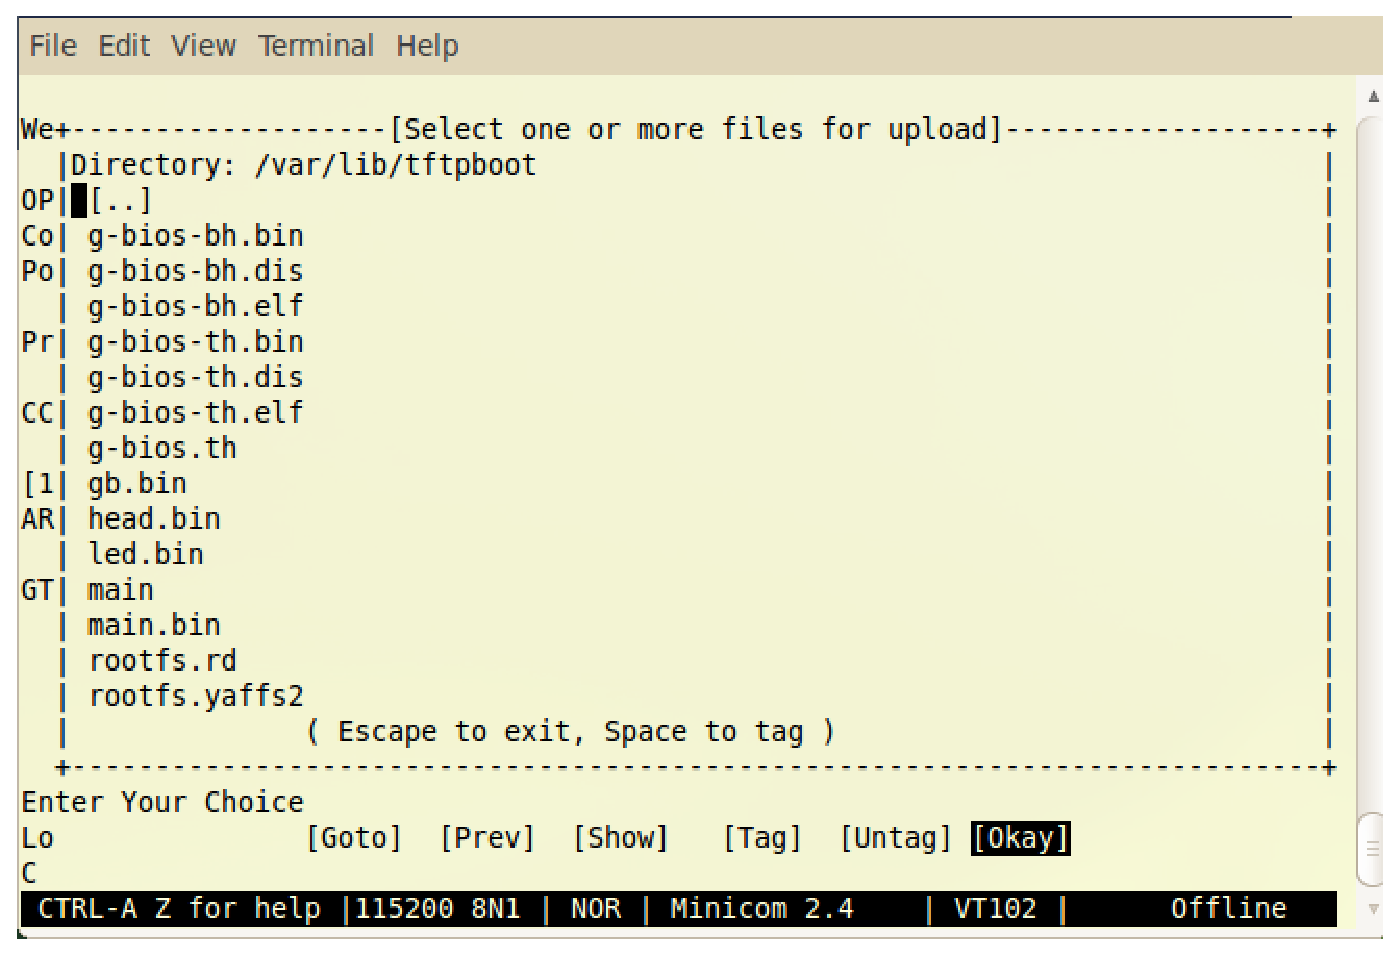
\includegraphics[width=0.8\textwidth]{image/min_05.eps}
		\end{figure}
	\item 输入/var/lib/tftpboot/g-bios.bin。回车。此处输入的为g-bios.bin文件的路径,可视具体情况更改。
		\begin{figure}[H]
		\centering
		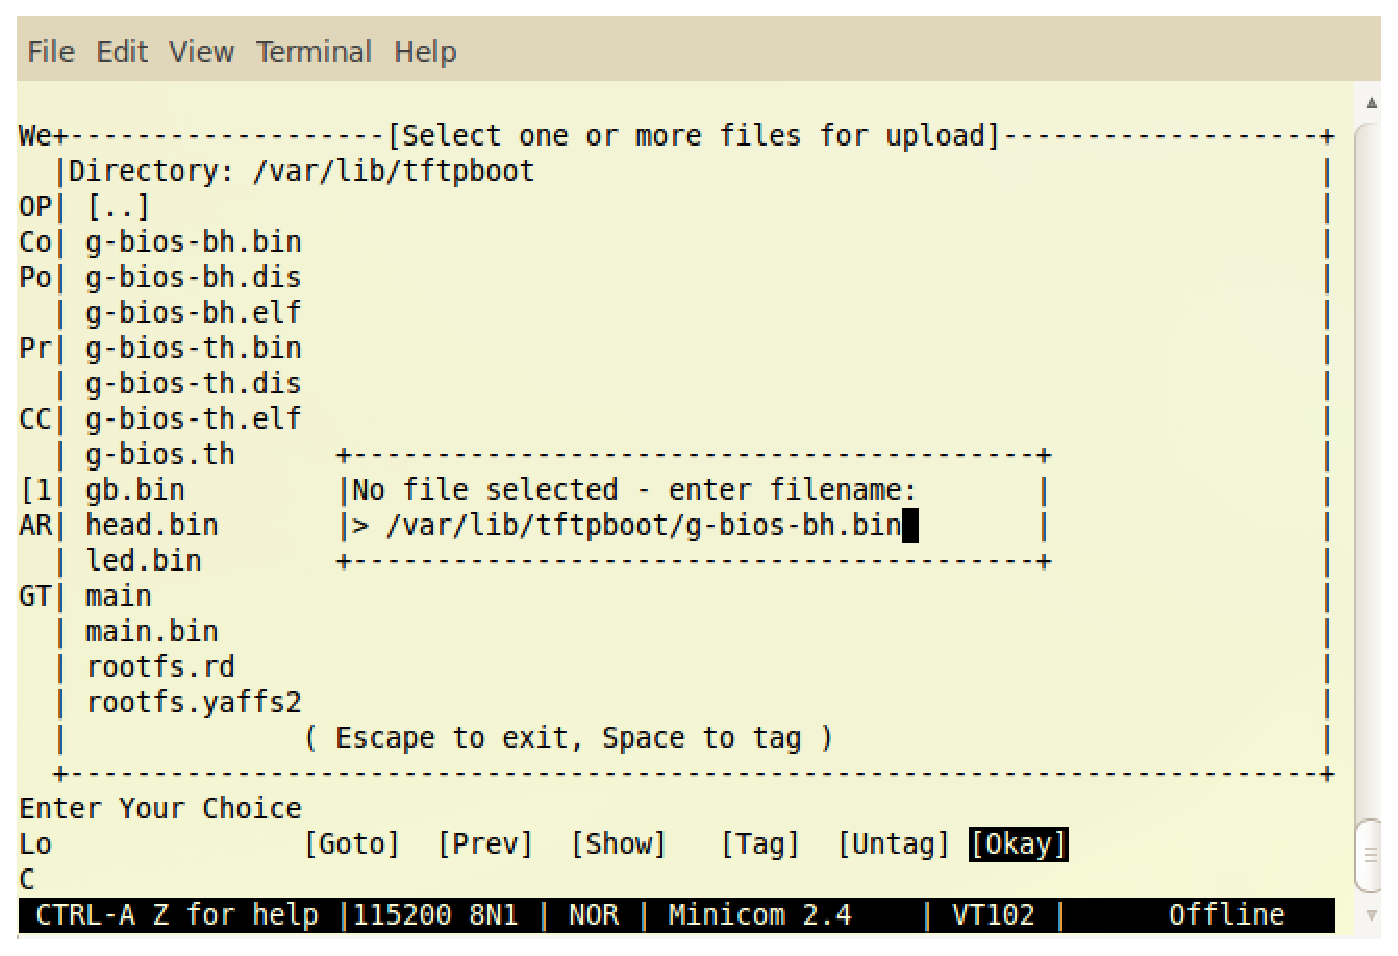
\includegraphics[width=0.8\textwidth]{image/min_06.eps}
		\end{figure}
	\item 开发传输文件,传送完成后如下图所示。再次回车。即可进入g-bios Shell。
		\begin{figure}[H]
		\centering
		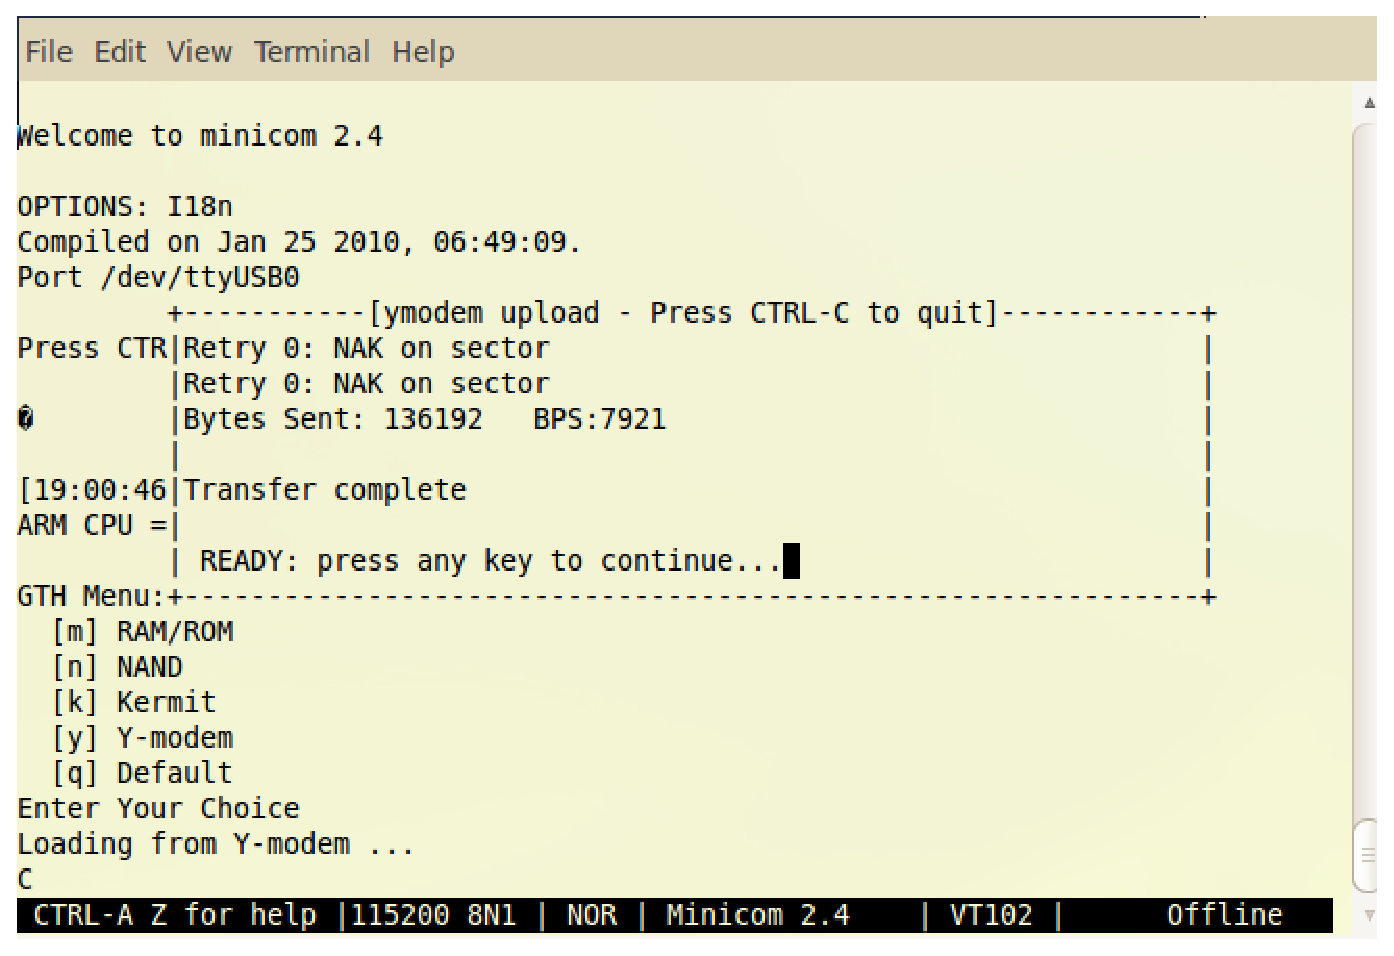
\includegraphics[width=0.8\textwidth]{image/min_07.eps}
		\end{figure}
	\item 进入g-bios Shell。如图所示。
		\begin{figure}[H]
		\centering
		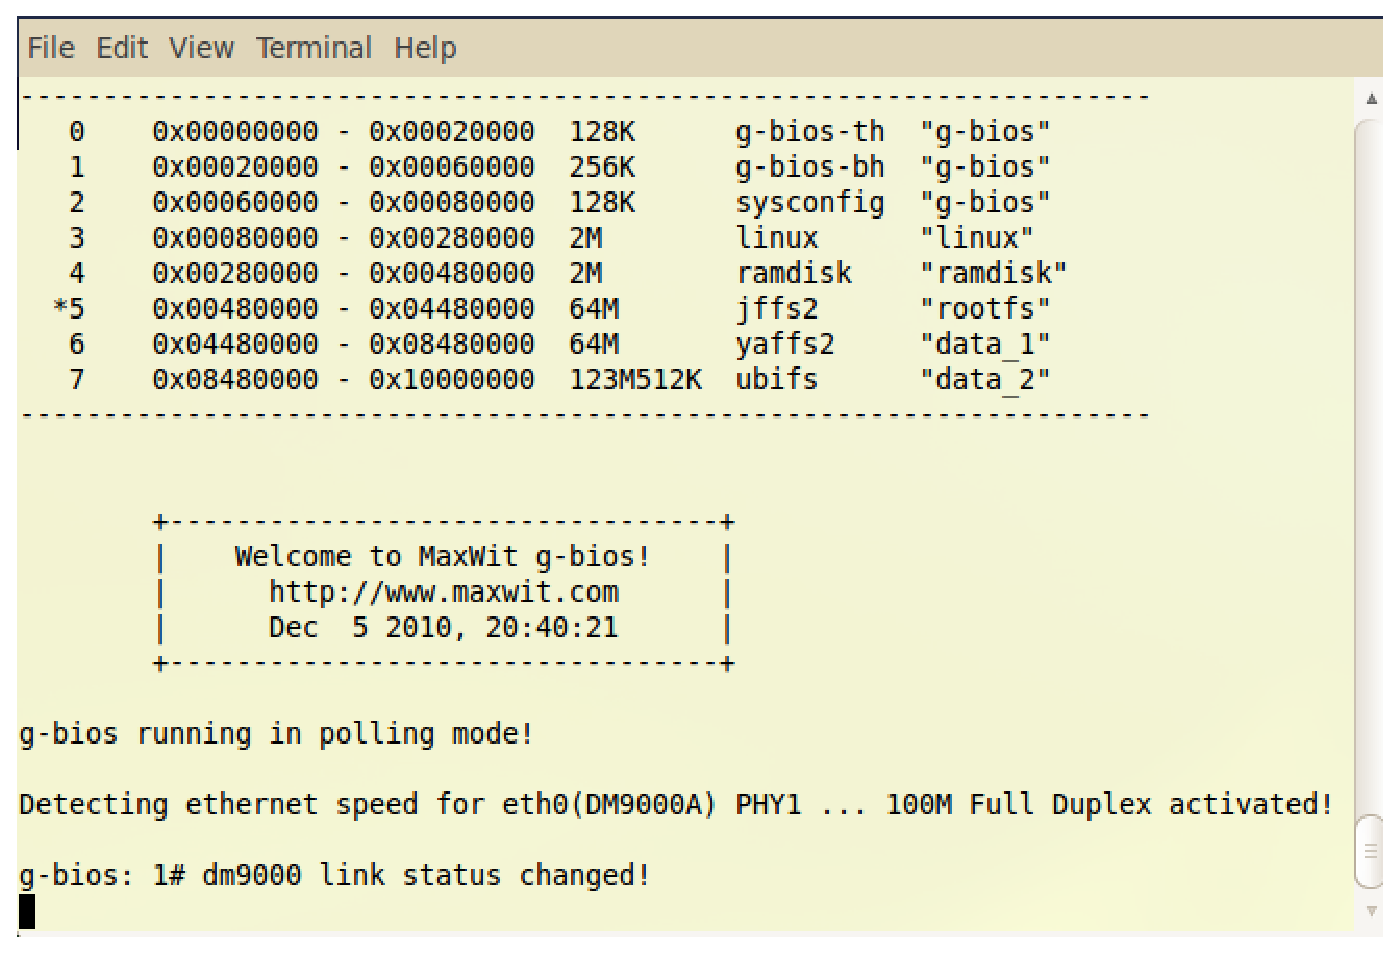
\includegraphics[width=0.8\textwidth]{image/min_08.eps}
		\end{figure}

	如果上述操作失败,以返回第三步(c步)重复操作,在第'f'步,不再重新输入,而是直接回车。
	\end{enumerate}
\item Kermit
\end{enumerate}
\noindent{}第一步,先启动上半部,使用串口线将开发板上的COM1口和PC机的COM口连接、并用网线连接开发板和PC机,在Host端打开kermit\\
\begin{lstlisting}[language=bash,escapeinside=``]
$cd /var/lib/tftpboot
$kermit
C-kermit>c (`回车`)
\end{lstlisting}
\noindent{}第二步,再按下开发板Reset键,将会进入g-bios上半部的启动界面(如图)\\

\begin{figure}[t]
\centering
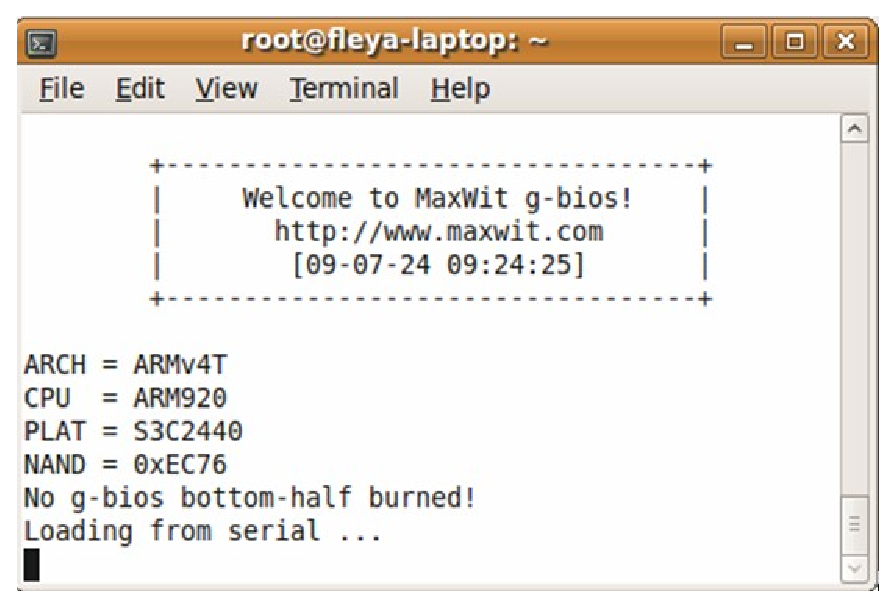
\includegraphics[width=5in]{image/step2.eps}
\end{figure}

\noindent{}注:g-bios的上半部会自动检测Flash上是否已烧录下半部g-bios.bin,若下半部已烧录则直接从Flash上将下半部Load到Sdram并运行,若未烧录则如上图所示,提示下半部未烧录,并需要通过从串口Load下半部并启动。下半部支持通过网络和串口两种方式烧录指定文件到Flash中。也在上半部启动过程中按任意键启动串口Load的功能.

\noindent{}第三步,选择``k''回车, 然后同时按下``CTRL''和``\textbackslash''键, 再按下``c''\\

\begin{figure}[H]
\centering
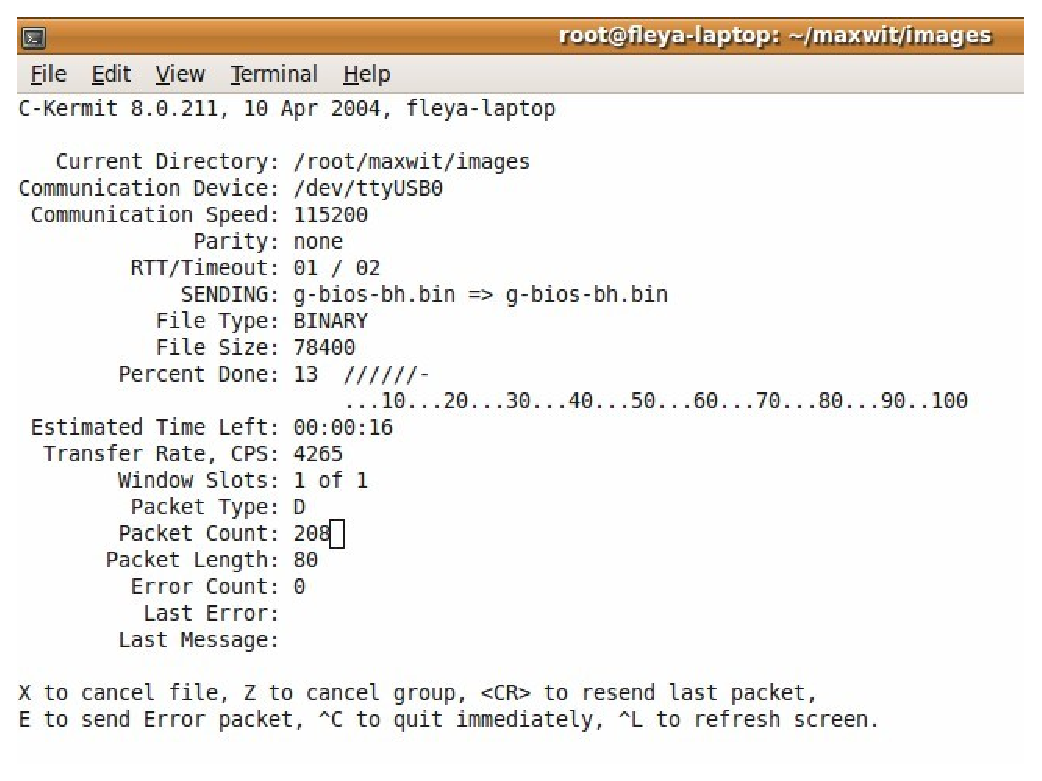
\includegraphics[width=5in]{image/step3.eps}
\end{figure}

\begin{lstlisting}[language=bash,numbers=none]
C-Kermit> send g-bios.bin
\end{lstlisting}
进入g-bios下半部的启动界面,按任意键进入g-bios的命令行,否则g-bios将会自动load kernel并启动(如图)

\begin{figure}[H]
\centering
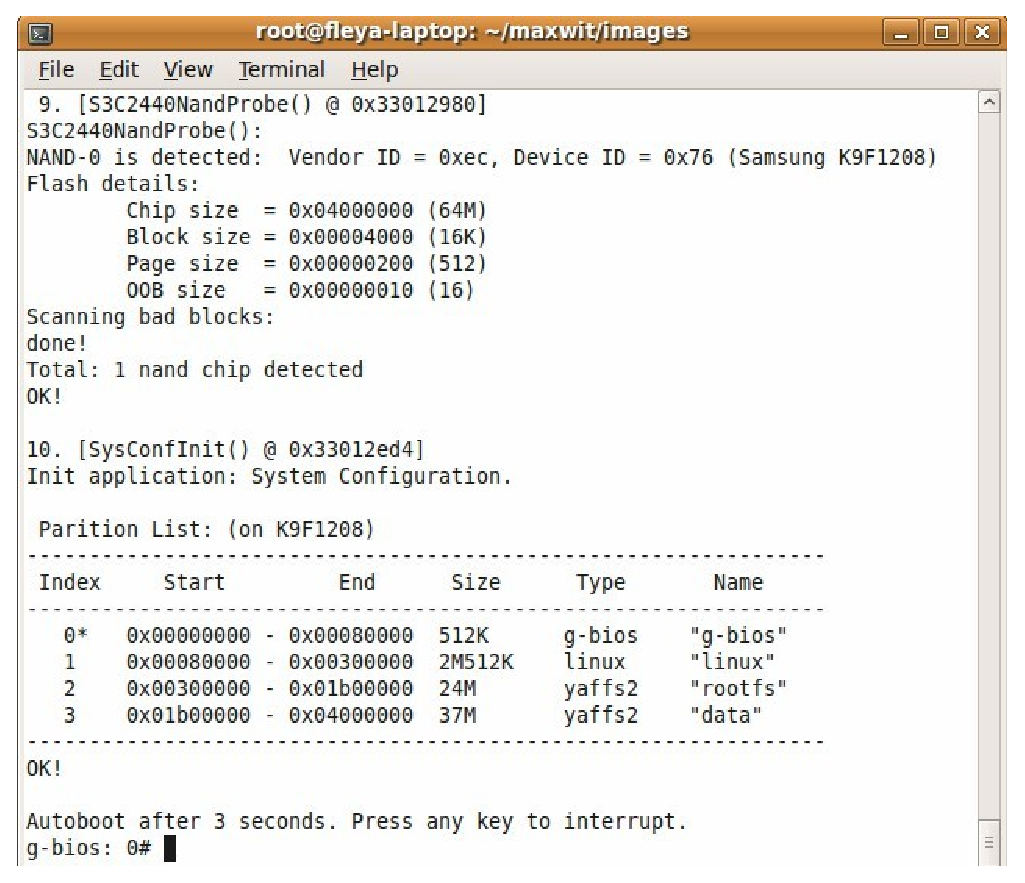
\includegraphics[width=5in]{image/step4.eps}
\end{figure}

\subsection{串口}
\subsection{SD卡}
\subsection{网络}

\begin{enumerate}
\item Write TH Image to SD Card
\item Booting g-bios TH from SD
\item Load BH to RAM
\item Burning TH and BH
\end{enumerate}


\chapter{g-bios命令详解}
\section{flash读写及分区}
\subsection{flash}
usage: flash <子命令> [可选参数 <值>]

\begin{table}[H]
%\centering
\setlength{\parindent}{0pt}
\begin{tabular}{|c|l|} \hline
子命令名称 & 命令说明 \\ \hline
%select & 选中某个flash设备,作为其他flash命令的操作对象 \\ \hline
dump & 查看flash页内容,以page为单位,包括oob \\ \hline
read & 从Flash中加载数据到DDR \\ \hline
write & Flash中写数据from DDR \\ \hline
erase & 以block为单位,擦除flash一块内容 \\ \hline
scanbb & 扫描指定分区上的坏快 \\ \hline
\end{tabular}
%\caption{Flash子命令}
\end{table}

\begin{table}[H]
\setlength{\parindent}{0pt}
\begin{tabular}{|c|l|} \hline
参数 & 功能 \\ \hline
-a & 设定起始地址\\ \hline
-l & 设定长度\\ \hline
-p & 设定分区,不与-a和-l并用\\ \hline
-m & mem的起始址址\\ \hline
-f & 强制erase(无论是否存在坏块)\\ \hline
-c & 擦除的同时写入cleanmark\\ \hline
\end{tabular}
\end{table}

命令使用示例:\\
\begin{itemize}
\item flash erase -a 1M -l 32K
\item flash erase -a 100block -l 16block -f
\end{itemize}

\subsection{part}
usage: part [options]

参数说明:

\begin{table}[H]
\begin{tabular}{|c|l|}
\hline
参数 & 功能 \\ \hline
-l & 显示分区表 \\ \hline
%-i [N] & 显示分区N的具体信息 \\ \hline
\end{tabular}
\end{table}

\subsection{ls}
显示当前分区的具体信息

\subsection{cd}
切换分区

\section{MMC/SD卡操作}
\subsection{mmc}
usage: mmc $<$子命令$>$ [options]

\begin{table}[H]
%\centering
\setlength{\parindent}{0pt}
\begin{tabular}{|c|l|} \hline
子命令名称 & 命令说明 \\ \hline
scan & 扫描所有MMC/SD设备,解析并打印设备信息 \\ \hline
%select & 选中某个MMC/SD设备,作为其他MMC/SD命令的操作对象 \\ \hline
dump & 查看MMC/SD上的数据,每次显示一个block \\ \hline
%read & 从MMC/SD中加载数据到DDR \\ \hline
%write & MMC/SD中写数据from DDR \\ \hline
%erase & 以block为单位,擦除MMC/SD一块内容 \\ \hline
\end{tabular}
%\caption{MMC子命令}
\end{table}

MMC/SD命令选项及参数介绍:
\begin{table}[H]
\setlength{\parindent}{0pt}
\begin{tabular}{|c|l|} \hline
参数 & 功能 \\ \hline
-a & 设定起始地址\\ \hline
%-l & 设定长度\\ \hline
%-m & mem的起始址址\\ \hline
\end{tabular}
\end{table}

\section{网络连接}

\subsection{ifconfig}
usage: ifconfig [interface] [address] [netmask <address>] [hw [HW] <address>]

选项及参数介绍:
\begin{table}[H]
\setlength{\parindent}{0pt}
\begin{tabular}{|l|l|} \hline
选项 & 功能描述 \\ \hline
interface & 指定网络设备对象,如``eth0''。缺省为系统中第一个网络设备。 \\ \hline
address & 配置网络设备IP地址为address \\ \hline
netmask <address> & 配置netmask为address \\ \hline
hw [HW] <address> & 配置设备的MAC地址为address。其中HW缺省为``ether'' \\ \hline
\end{tabular}
\end{table}

不加任何option时显示interface的信息,具体包括:
\begin{enumerate} \setlength{\itemsep}{-\itemsep}
\item NIC芯片名称(ID及字符串表示)
\item PHY信息:ID、地址
\item 连接状态,包括速率
\item RX/TX bytes
\item error count
\end{enumerate}

\subsection{ping}
usage:ping [DestIp] 

若DestIp不指定,则默认的server ip

\subsection{tftp}
usage:tftp [options] [filename]

参数介绍:
\begin{table}[H]
\setlength{\parindent}{0pt}
\begin{tabular}{|c|l|} \hline
选项 & 功能描述 \\ \hline
 -s & 设定服务端IP \\ \hline
 -m & 下载的内容放在内存里,即,不烧录到flash上 \\ \hline
\end{tabular}
\end{table}

\subsection{dhclient}
usage:dhclient [options]

参数介绍:
\begin{table}[H]
\setlength{\parindent}{0pt}
\begin{tabular}{|c|l|} \hline
选项 & 功能描述 \\ \hline
 -s & 同时将Server IP更新为DHCP Server \\ \hline
\end{tabular}
\end{table}

\section{串口协议及工具}

\subsection{kermit}
usage:kermit [options]

作用概述:串口文件传输%\footnote{目前kermit和ymodem仅支持下载}

选项及参数介绍:
\begin{table}[H]
\setlength{\parindent}{0pt}
\begin{tabular}{|c|m{10cm}|} \hline
选项 & 功能描述 \\ \hline
 -m [address] & 将下载的数据放在内存中,而不直写到storage(如Flash)上。其中address为可选参数,表示memory地址;若不指定address,则由系统自动分配一块空间。 \\ \hline
\end{tabular}
\end{table}

\subsection{ymodem}
usage: ymodem [options]

作用概述:串口文件传输%\footnote{目前kermit和ymodem仅支持下载}

选项及参数介绍:
\begin{table}[H]
\setlength{\parindent}{0pt}
\begin{tabular}{|c|m{10cm}|} \hline
选项 & 功能描述 \\ \hline
 -m [address] & 将下载的数据放在内存中,而不直写到storage(如Flash)上。其中address为可选参数,表示memory地址;若不指定address,则由系统自动分配一块空间。 \\ \hline
\end{tabular}
\end{table}

\section{Graphics和Display}
\subsection{lcd}
usage:lcd [options]

参数介绍:
\begin{table}[H]
\setlength{\parindent}{0pt}
\begin{tabular}{|c|l|} \hline
选项 & 功能描述 \\ \hline
-l [all] & 列出LCD的video mode。all表示所有video mode,不加则仅显示当前的video mode \\ \hline
-s <N> & 将当前LCD的video mode设置为第N种mode。 \\ \hline
\end{tabular}
\end{table}

\section{memory读写及指令跳转}

\subsection{mem}
\begin{table}[H]
%\centering
\begin{tabular}{|c|l|}
\hline
命令名称 & 命令说明\\ \hline
read & 显示memory数据\\ \hline
write & 将数据写入memory\\ \hline
set & 将某个memory空间写入值\\ \hline
\end{tabular}
%\caption{md}
\end{table}

\subsection{go}
usage: go <address>

address跳转的目标地址,可十进制表示,也可十六进制表示。

示例: go 0xc000000 跳转到0xc000000处执行。

\section{系统配置}
\subsection{sysconf}
\begin{table}[H]
%\centering
\begin{tabular}{|c|l|}
\hline
命令名称 & 命令说明\\ \hline
-r <all|net|boot> & sysconf reset \\ \hline
\end{tabular}
%\caption{md}
\end{table}

\section{其他命令}
\subsection{help}
列出g-bios系统中当前所有可用的命令

\subsection{led}
LED灯测试


\chapter{引导操作系统}

%\section{Add New Commands}
%g-bios添加命令规范。
%\begin{lstlisting}
%static char app_option[][CMD_OPTION_LEN] = {};
%
%#include <getopt.h>
%
%int getopt(int argc, char *argv[], const char *optstring, char **arg);
%\end{lstlisting}

boot command design ..

\section{OS引导}
见第五章?
\begin{table}[H]
\setlength{\parindent}{0pt}
\begin{tabular}{|c|c|}
\hline
 命令名称 & 命令说明\\
\hline
boot & 引导操作系统\\
\hline
\end{tabular}
\end{table}

\noindent{}命令名称:boot\\
参数介绍:\\
\begin{table}[H]
\setlength{\parindent}{0pt}
\begin{tabular}{|p{2.5cm}|p{8.5cm}|}
\hline
-t [filename] &若指定filename,则通过tftp下载kernel image文件;否则从本地的linux分区下载kernel image文件 \\ \hline
-r [filename] &用ramdisk启动。指定filename,则通过tftp下载ramdisk image;否则从本地ramdisk分区下载。 \\ \hline
-f [N] & 指定rootfs分区,N为分区号 \\ \hline
-n [ip:path] & 用nfs方式mount rootfs \\ \hline
-v &仅显示kernel启动参数,但并不真正引导OS \\ \hline
\end{tabular}
\end{table}
\section{TFTP + NFS}

\indent 其中NFS服务配置和编译linux kernel部分详情请参阅$<<$MaxWit Lablin开发者手册$>>$第一卷\\
\indent 在g-bios命令行下,输入:\\

\begin{verbatim}
g-bios: 0# boot -t zImage -n 192.168.0.2:/home/maxwit/maxwit/rootfs
【说明】
-t [filename]:用tftp方式下载指定的kernel image
-n [nfs_server:/nfs/path/]: 用NFS方式mout rootfs。也可以加上参数,如:-n 192.168.0.111:/path/to/nfs
\end{verbatim}

boot程序具有记录功能,即,能记住用户输入的参数,换句话,再次输入boot时不再需要输入参数了,除非你想重设参数。

\section{FLASH + NFS}
\begin{verbatim}
g-bios: 1# cd 3  (进入Linux分区)
g-bios: 3# ls (列出当前分区信息)
        Partition Type = "linux"
        Partition Base = 0x00080000 (512K)
        Partition Size = 0x00200000 (2M)
        Host Device    = NAND 256MB 3.3V 8-bit
        MTD Deivce     = /dev/mtdblock3
        Image File     = "zImage" (1968220 bytes)
g-bios: 3# tftp zImage (下载zImage 到当前分区)
 "zImage": 192.168.2.101 => 192.168.2.100
 1968220(1M898K92B) loaded

g-bios: 1# boot  -t  -n 192.168.2.11:/root/maxwit/rootfs
【说明】
-t  不加参数,从Linux分区Load kernel image
-n [nfs_server:/nfs/path/]: 用NFS方式mount rootfs。也可以加上参数。如:-n 192.168.0.111:/home/maxwit/maxwit/rootfs。
\end{verbatim}

\section{Booting from Flash}

\begin{verbatim}
g-bios: 1# cd 3  (进入Linux分区)
g-bios: 3# ls (列出当前分区信息)
        Partition Type = "linux"
        Partition Base = 0x00080000 (512K)
        Partition Size = 0x00200000 (2M)
        Host Device    = NAND 256MB 3.3V 8-bit
        MTD Deivce     = /dev/mtdblock3
        Image File     = "zImage" (1968220 bytes)
g-bios: 3# tftp zImage (下载zImage 到当前分区)
 "zImage": 192.168.2.101 => 192.168.2.100
 1968220(1M898K92B) loaded

g-bios: 3# cd 5 (进入Rootfs分区)
g-bios: 5# tftp rootfs_l.jffs2 (下载zImage 到当前分区)
g-bios: 5# boot -t -f 5
【说明】
-t :不加参数,从Linux分区Load kernel image
-f [N]:指定rootfs的分区,N为分区号
\end{verbatim}


\chapter{附录I:虚拟机下g-bios烧录方式举例}
\section{Qemu虚拟环境}

\subsection{思路分析}
\begin{enumerate}
	\item 环境配置:
	\begin{itemize}
		\item Qemu
		\item Serial tools: minicom/kermit
	\end{itemize}

	\item g-bios load 机制:
	\begin{itemize}
		\item th load bh
		\item bh load sysconfig and linux kernel.
	\end{itemize}
	th 启动成功后,接着检测 bh,如果检测成功即启动 bh 部分,反之则会等待 bh 的烧录(有时间限制); g-bios 目前支持4种方式的 bh load。

	\item 步骤分析:
	\begin{itemize}
		\item 虚拟一块存储介质,将 g-bios th 部分烧录进该虚拟介质(目前 g-bios 已经支持 nand flash image 的制作);
		\item 利用虚拟机从该介质启动,并进入 g-bios th 启动菜单界面;
		\item 此时即可根据菜单提示尽情折腾了...
	\end{itemize}
\end{enumerate}

\subsection{具体实例}
本例采用 mw71 作为虚拟开发板,其他板子方法类似。
\begin{enumerate}
	\item 编译 g-bios: \\
	g-bios 中进入 th load 引导菜单可以通过长按键盘空格键进入,这在硬件平台上是完全可以做到的,但是由于虚拟机的启动比较快,很难做到(多次试验失败)。\\
	可以通过修改 g-bios th load 部分代码来达到目的。\\
	具体修改文件为:g-bios/th/base/main.c
	\lstset{language=[ANSI]C}
	\begin{lstlisting}[numbers=none]
		...
	37	// for(i = 0; i < 0x100; i++)
	38	while (1)
		...
	\end{lstlisting}
	修改OK后,按如下步骤编译:
	\begin{lstlisting}[language=sh,numbers=none]
	$ make mw71_defconfig
	$ make
	$ make install  // install g-bios image to /var/lib/tftpboot
	\end{lstlisting}

	\item 制作 image:
	\begin{lstlisting}[language=csh,numbers=none]
	$ cp build/simulators/omap3530/bb_nandflash.sh /var/lib/tftpboot
	$ ./bb_nandflash.sh witrom.bin mw_flash.img
	\end{lstlisting}
	在此 image 中只烧录 g-bios 的 th 部分。

	\item 运行:
	\begin{lstlisting}[language=csh,numbers=none]
	$ qemu-system-arm -M mw71 -mtdblock mw_flash.img -serial pty
	\end{lstlisting}
	得到如下信息:
	\begin{lstlisting}[numbers=none]
	0+1 records out
	1004 bytes (1.0 kB) copied, 4.2184e-05 s, 23.8 MB/s
	put bl1 into flash image done!
	char device redirected to /dev/pts/5
	\end{lstlisting}
	根据上面的启动信息,设置 minicom 配置参数( kermit 类似)。
	\begin{lstlisting}[language=csh,numbers=none]
	$ cat ~/.minirc.dfl
	# Machine-generated file - use setup menu in minicom to change parameters.
	pu port             /dev/pts/5
	\end{lstlisting}
	敲入如下命令,待 minicom 启动后敲任意键,即可得到 th 启动界面。
	\begin{lstlisting}[language=csh,numbers=none]
	$ sudo minicom
	\end{lstlisting}
	接下来进入那比较熟悉的界面,th 部分的 load 方式可以很容易的进行尝试。

\end{enumerate}

\section{Others}


\chapter{附录II:具体硬件平台g-bios烧录方式举例}
\section{S3C24XX系列平台}

\section{AT91SAM系列平台}

\section{S3C64XX系列平台}
S3C64XX and S5P as cases

\section{OMAP3系列平台}
\subsection{devkit8000开发板}
将g-bios烧录到SD卡的步骤如下:
\begin{enumerate}
\item make devkit8000\_defconfig
\item make
\item make install将witrom.bin以及g-bios.bin拷贝到默认目录/var/lib/tftpboot下
\item 将SD卡插入PC,创建一个fat32分区,并将其设置为启动分区,具体步骤如下:
 \begin{enumerate}
  \item 依据读卡器的不同,sd卡插入后会在dev目录下产生sdb或者mmcblk0文件,执行如下命令sudo fdisk /dev/sdb或者/dev/mmcblk0
  \item 依照提示,按下n(add a new partition)
  \item 按下p键(创建primary partition)
  \item 按下1
  \item 一路回车
  \item 按下a键(toggle a bootable flag)
  \item 按下1
  \item 按下t键(change a partition's system id)
  \item 按下l键
  \item 选择c(W95 FAT32(LBA))
  \item 按下w键
  \item 按下q键退出fdisk
  \item 执行如下命令:sudo mkfs.vfat /dev/sdb1或者/dev/mmcblk0p1,将分区格式成FAT32
 \end{enumerate}
\item 将sd卡上的FAT32分区mount到pc上后,将witrom.bin拷贝到sd的FAT32分区上,并将其改名为MLO文件
\item umount sd卡
\end{enumerate}
从SD卡启动方法如下:
将SD插入开发板,按住boot键,开启电源(此时是从SD卡启动,若直接开启电源,则从NAND启动)


\end{document}
